\section{Evaluation}
\label{s:eval}

\begin{figure*}
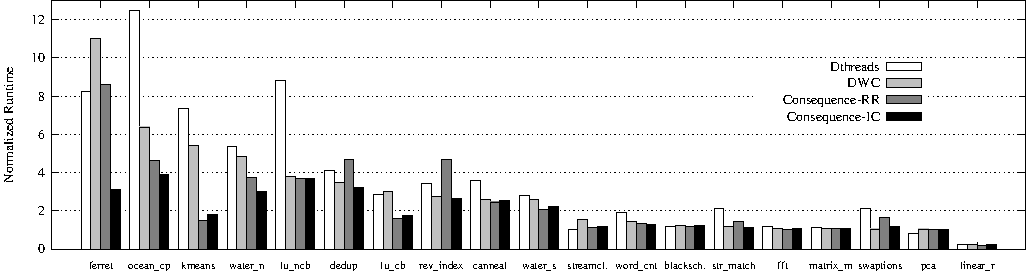
\includegraphics[width=6.0in]{figures/overall_runtimes.pdf}
\caption{\lib{} and DThreads runtime scaled to pthreads runtime (best result for all libraries).}
\label{f:performance}
\end{figure*}


\begin{figure*}
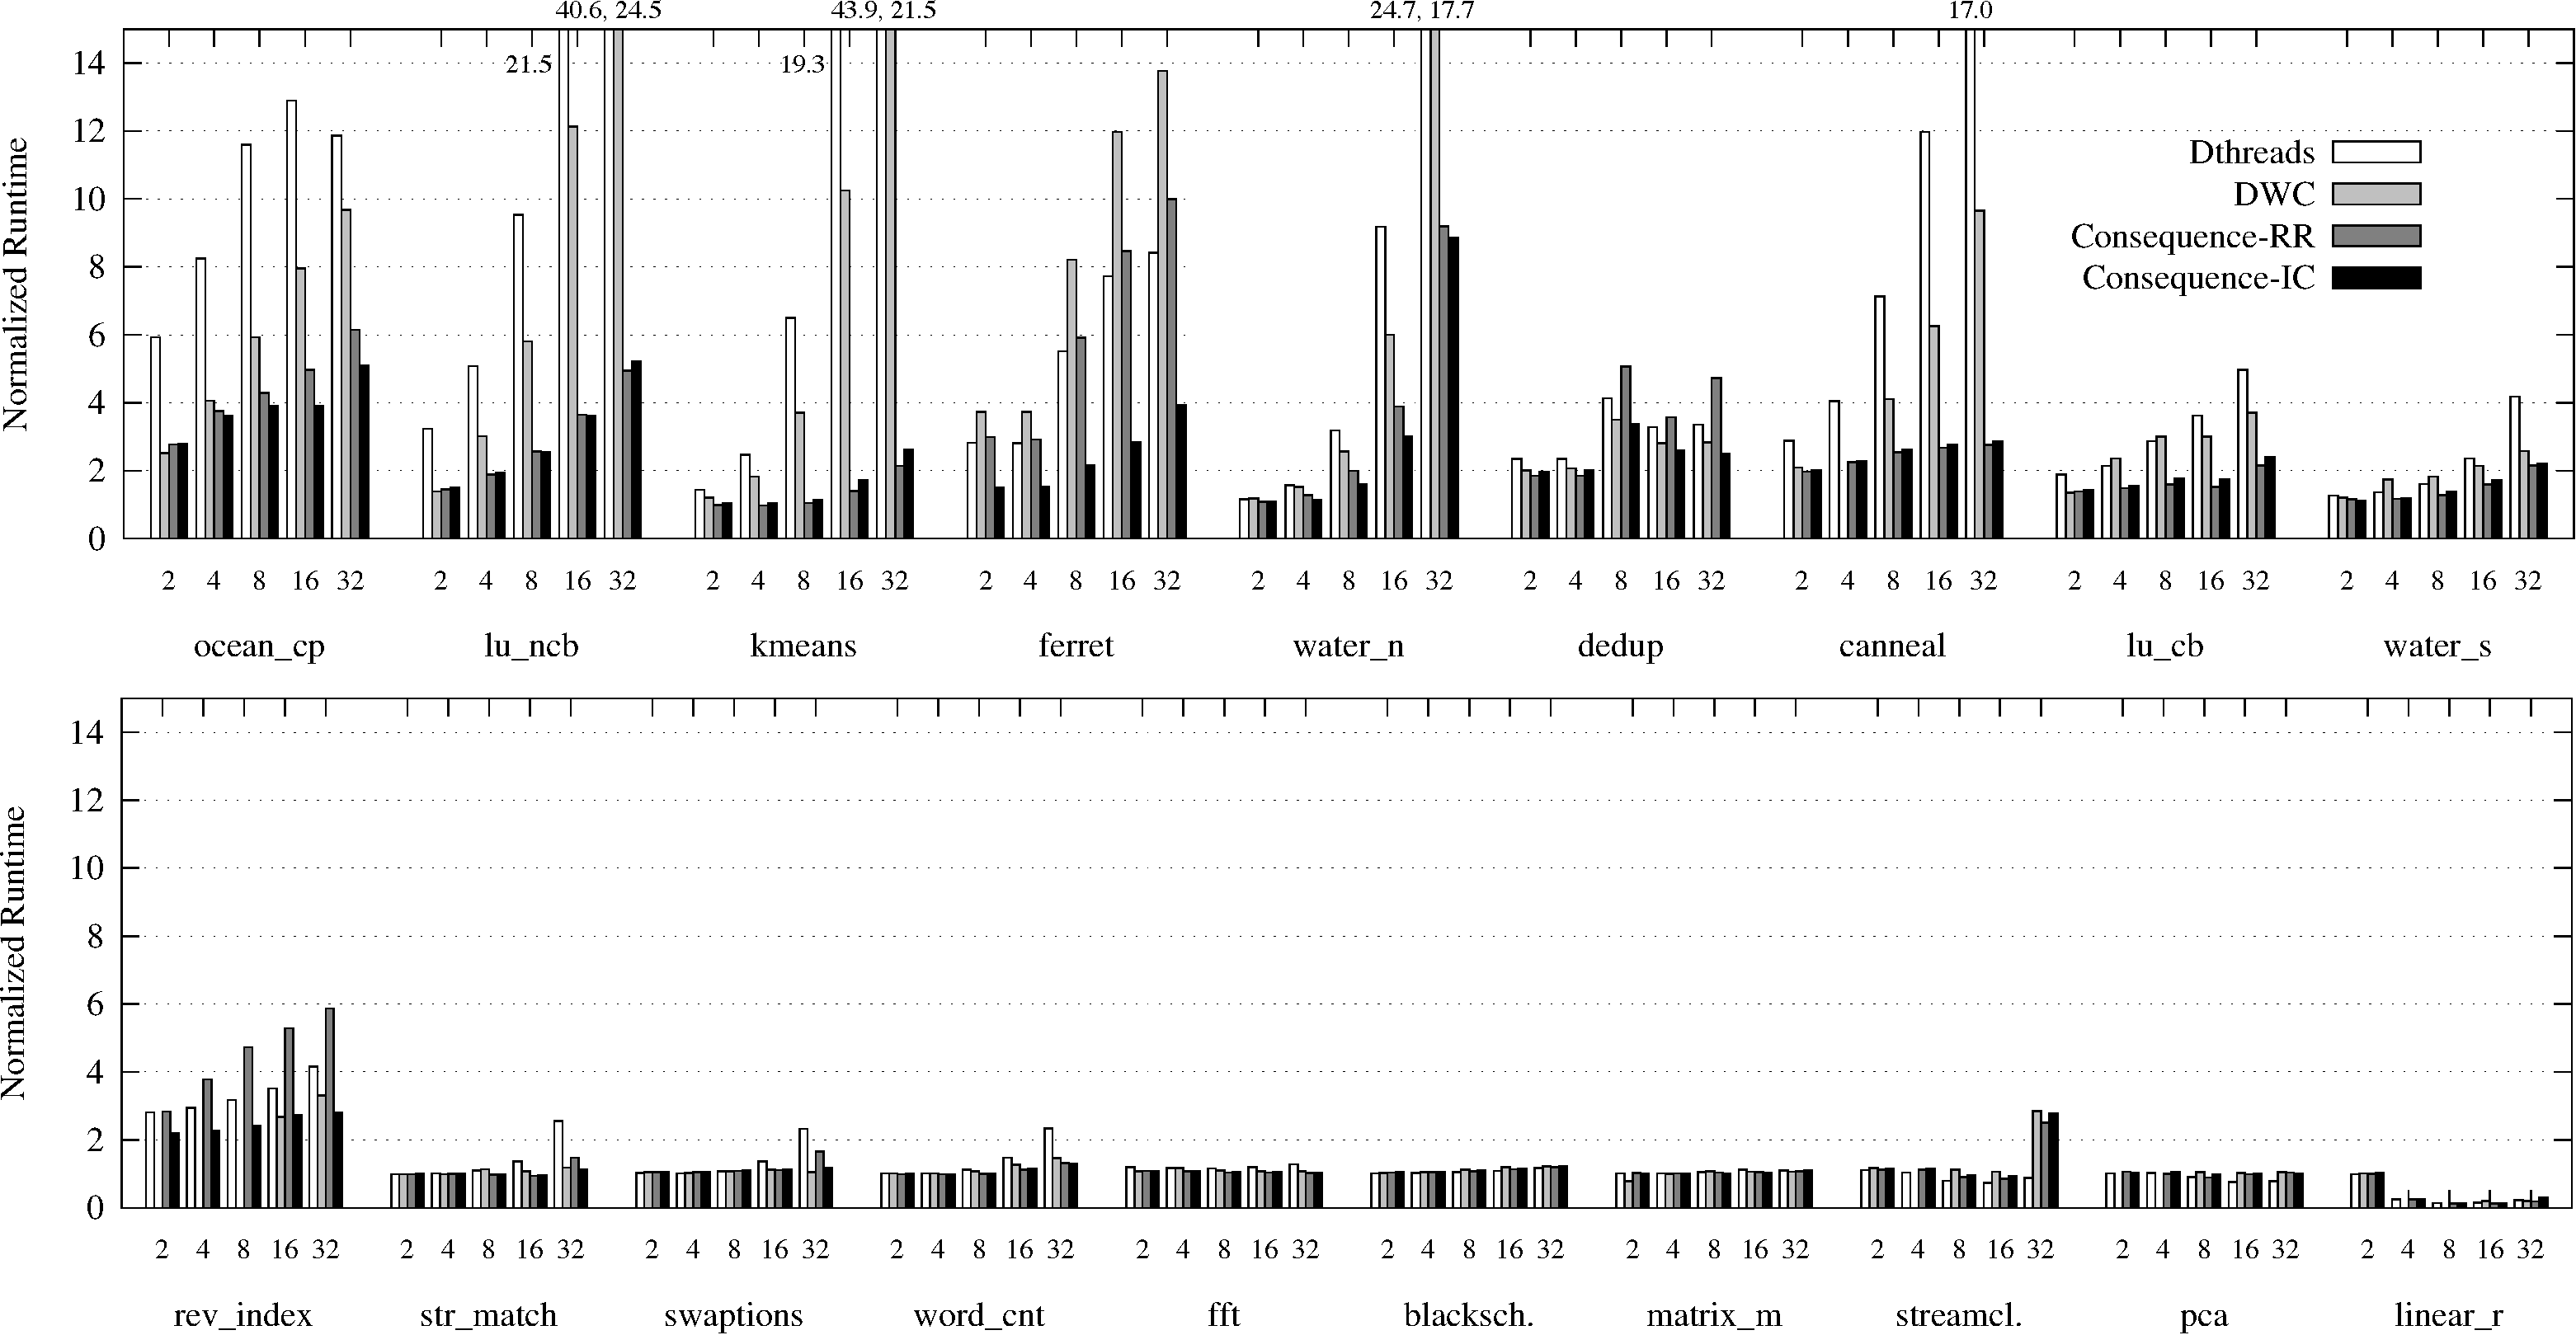
\includegraphics[width=6.4in]{figures/scalability_results.pdf}

\caption{Performance when varying the number of threads for \lib{} and DThreads (normalized to pthreads).}
\label{f:scalability}
\end{figure*}


\begin{figure*}
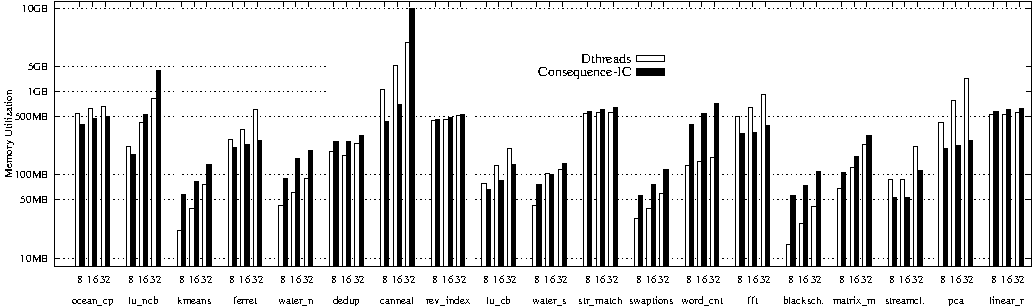
\includegraphics[width=6.4in]{figures/memory_utilization.pdf}
\caption{Total memory usage for {\lib{} and DThreads (normalized to pthreads).}}
\label{f:memory}
\end{figure*}



\begin{figure}
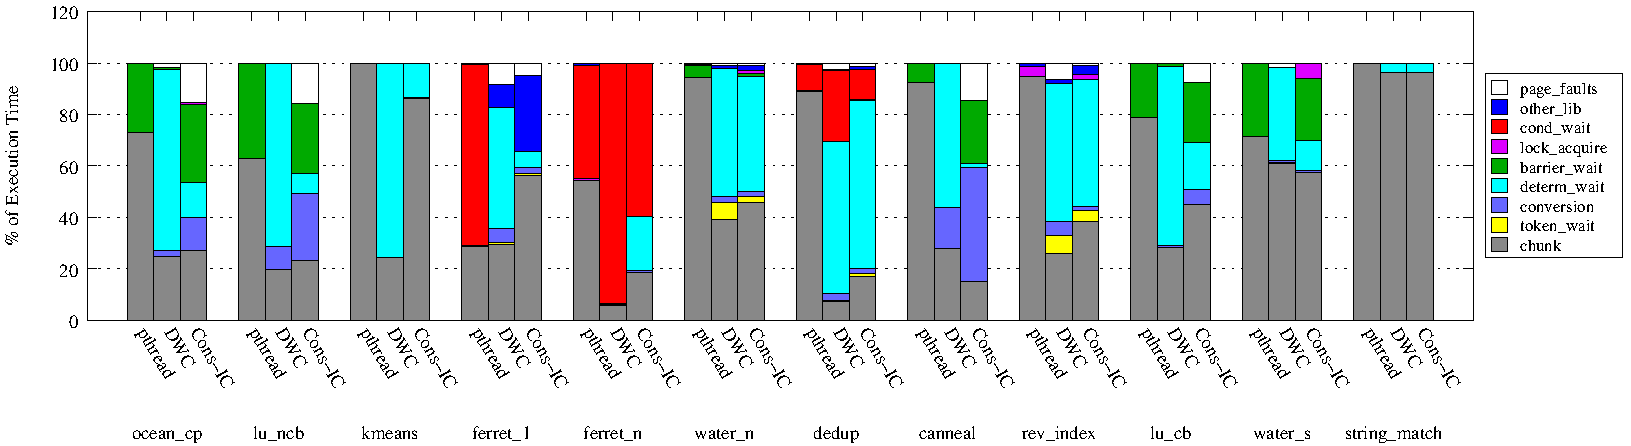
\includegraphics[width=3.0in]{figures/fine_grained_analysis.pdf}
\caption{}
\label{f:fine-grained}
\end{figure}


\begin{figure}
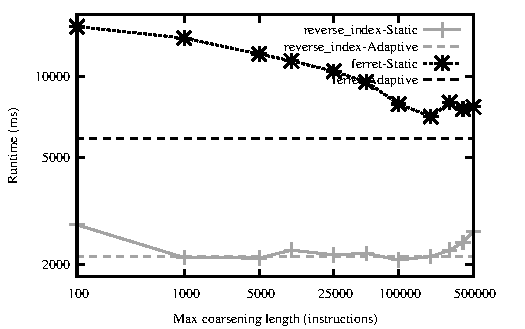
\includegraphics[width=3.0in]{figures/adaptive.pdf}
\caption{}
\label{f:adaptive}
\end{figure}


\begin{figure}
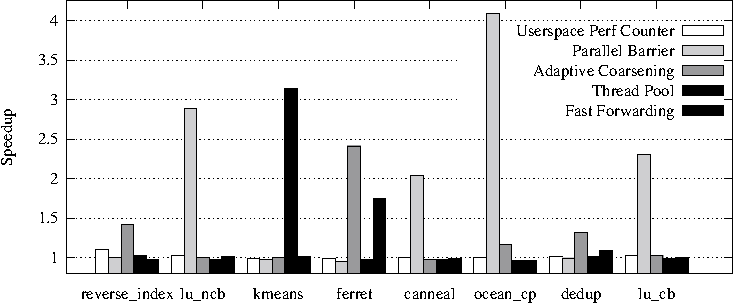
\includegraphics[width=3.0in]{figures/optimizations.pdf}
\caption{}
\label{f:adaptive}
\end{figure}

\subsection{Comparison with RFDet}

<<<<<<< .mine
RFDet\cite{rfdet} is a recent proposal for a deterministic multi-threading library using LRC. While the paper reported strong performance on SPLASH-2 and Parsec benchmarks, the evaluation was limited to low thread counts for more intensive benchmarks due to very high memory consumption.
=======
We contacted the authors of RFDet \cite{kai_lu_efficient_2014} in an effort to compare \lib{} against the state of the art in LRC determinism. A version of the RFDet implementation was provided to us by the authors, the results of which are presented below. Despite our best efforts, and several requests for the actual code used for \cite{kai_lu_efficient_2014} and assistance in reproducing their results, we were unable to acquire or re-create a correct implementation. Among our concerns are:
>>>>>>> .r401

<<<<<<< .mine
Unfortunately, the currently available implementation of RFDet is provided without deterministic synchronization, which was described in the paper as an implementation of Kendo using compiler instrumentation to provide logical time (instead of performance counters). Further, of the 12 Parsec and Phoenix benchmarks we experimented with, we could only obtain error-free executions for 4 of them.
=======
First, the implementation we were provided fundamentally does not provide determinism: RFDet as described depends on Kendo \cite{olszewski_kendo:_2009} for synchronization, but this is not implemented. In the paper, the authors claim to have ``implemented'' Kendo, which would be a significant engineering effort. This discrepancy was not adequately addressed by the authors despite multiple requests from us. \TODO{wasn't there something about synch op implementations missing clock calls too?}.  
>>>>>>> .r401

<<<<<<< .mine
=======
Second, only \textcolor{red}{three out of X} benchmarks ran to completion under the RFDet implementation provided to us, even in its present non-deterministic state. In \cite{kai_lu_efficient_2014}, results from 16 benchmarks are reported. 

While it is possible that the results presented in \cite{kai_lu_efficient_2014} are an accurate representation of the author's evaluation experience, the lack of reproducibility, and the unwillingness of the authors to share their correct implementation, lends serious doubt to the claims made. 

>>>>>>> .r401
\begin{figure}
\centering
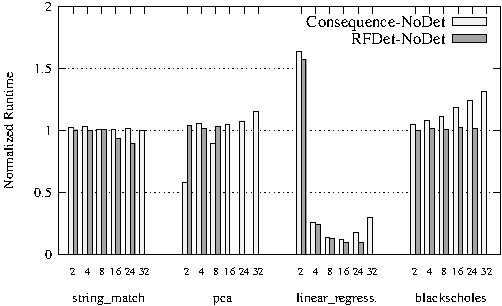
\includegraphics[width=3in]{figures/rfdet_perf}
\caption{Runtime performance of RFDet vs. \lib{} for the 4 benchmarks that ran to completion with RFDet.}
\label{f:rfdet}
\end{figure}


\begin{figure}
\centering
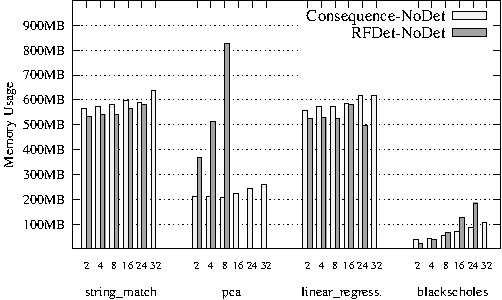
\includegraphics[width=3in]{figures/rfdet_mem}
\caption{Memory requirements of RFDet vs. \lib{}. Relaxed consistency models maintain more concurrent versions than total store order, sometimes resulting in significantly greater memory needs.}
\label{f:rfdet_memory}
\end{figure}

That said, Figure \ref{f:rfdet} shows the performance of the RFDet implementation provided to us, compared against \lib{}. In order to create an apples-to-apples comparison, we run \lib{} in non-deterministic mode (see \ref{f:deterministic-vs-nondeterministic} for a more extensive comparison of \lib{} performance in deterministic vs. non-deterministic TSO execution). The results of our limited experiments show that RFDet does not obtain a significant advantage over \lib{} for any of the 4 benchmarks evaluated. Though at higher thread counts RFDet tends to outperform \lib{}, we believe this is due to residual overhead from our GMIC module that has not been entirely removed from the \libnodet{} version. 

Figure \ref{f:rfdet_memory} compares the memory requirements of the two methods for the same set of benchmarks. For all but 3 benchmarks, RFDet and \lib{} have similar memory requirements. However, for the $pca$ benchmark, RFDet experiences a significant increase in memory utilization to due to a larger number of synchronization operations. The result is that RFDet is unable to complete the program error-free at higher thread counts.

In conclusion, while relaxed consistency models provide one possible path toward pthreads parity, more research is needed before this direction will produce practical and reproducible results. 
<<<<<<< .mine



%We contacted the authors of RFDet \cite{rfdet} in an effort to compare \lib{} against the state of the art in LRC determinism. A version of the RFDet implementation was provided to us by the authors, the results of which are presented below. Despite our best efforts, and several requests for the actual code used for \cite{rfdet} and assistance in reproducing their results, we were unable to acquire or re-create a correct implementation. Among our concerns are:

%First, the implementation we were provided fundamentally does not provide determinism: RFDet as described depends on Kendo \cite{kendo} for synchronization, but this is not implemented. In the paper, the authors claim to have ``implemented'' Kendo, which would be a significant engineering effort. This discrepancy was not adequately addressed by the authors despite multiple requests from us. \TODO{wasn't there something about synch op implementations missing clock calls too?}.  

%Second, only \textcolor{red}{three out of X} benchmarks ran to completion under the RFDet implementation provided to us, even in its present non-deterministic state. In \cite{rfdet}, results from 16 benchmarks are reported. 

%While it is possible that the results presented in \cite{rfdet} are an accurate representation of the author's evaluation experience, the lack of reproducibility, and the unwillingness of the authors to share their correct implementation, lends serious doubt to the claims made. 


=======

%%% Local Variables: 
%%% mode: latex
%%% TeX-master: "paper.tex"
%%% End:>>>>>>> .r401

